Allgemein ist zu sagen, dass es nicht einfach war einigermaßen plausible Ergebnisse zu erhalten.
Die Prozessorauslastung schwankte zumeist sehr stark, da viele Benutzer gleichzeitig auf den Maschinen testeten.
Aus diesem Grund kam es gelegentlich zu ungewöhnlich hohen Ausführungszeiten bei den parallelen Implementierungen, insbesondere bei Verwendung vieler Prozessoren.
Um dieses Problem abzuschwächen, ließen wir unsere Testsskripts mehrmals durchlaufen und warteten stets darauf, dass möglichst wenige Benutzer auf den Maschinen aktiv sind.

Wir haben zwei verschiedene Arten von Plots erstellt.
Zum einen wird die mittlere Ausführungszeit eines Tests als Funktion der Testgröße dargestellt.
Die Größe bezieht sich hierbei auf die Elemente eines einzelnen Arrays.
Das gemergte Array umfasst also doppelt so viele Elemente wie im Plot angegeben.
Zum anderen wird der erreichte Speedup als Funktion der Prozessorzahl visualisiert.

Der erreichte Speedup ist sehr stark von der Testgröße abhängig.
Sind die Arrays zu klein, ist der Synchronisations- bzw. Kommunikationsoverhead zu groß und es kann kein Nutzen aus der größeren Prozessorzahl gezogen werden.
Je mehr Prozesse resp. Threads beteiligt sind, desto größer wird der Overhead.
Bei einer sehr kleinen Arraygröße, wie 1000, kommt es daher bei allen parallelen Implementierungen zu einer deutlichen Verlangsamung im Vergleich zur sequentiellen Implementierung.
Erst ab einer Größe von etwa 100000 Elementen pro Array ist bei nahezu allen Implementierungen ein Geschwindigkeitsanstieg zu verzeichnen. 


\subsection{Cilk}
Mit Cilk konnten wir einen moderaten Speedup erzielen.
Aus den Abbildungen \ref{Cilk_Disjunct_sizes} und \ref{Cilk_Interleaved_sizes} ist ersichtlich, dass der Speedup bei ausreichend großen Testfällen anfangs schnell ansteigt, dann jedoch stagniert.
Wie zu erwarten, ist der Speedup bei komplett unabhängigen Arrays etwas größer als bei perfekt verzahnten.
Dennoch kamen wir selbst bei einer Testgröße von $n = 500000$ kaum über den Faktor 6 hinaus.
Eingedenk der Tatsache, dass der maximal mögliche Geschwindigkeitszuwachs bei 48 liegt, wirken die Ergebnisse der Cilk-Implementierung relativ bescheiden.
Eine grafische Übersicht der Benchmarks ist in den Abbildungen \ref{Cilk_Disjunct_sizes}, \ref{Cilk_Disjunct_cores}, \ref{Cilk_Interleaved_sizes} und \ref{Cilk_Interleaved_cores} zu finden.


\begin{figure}[p]
	\centering
	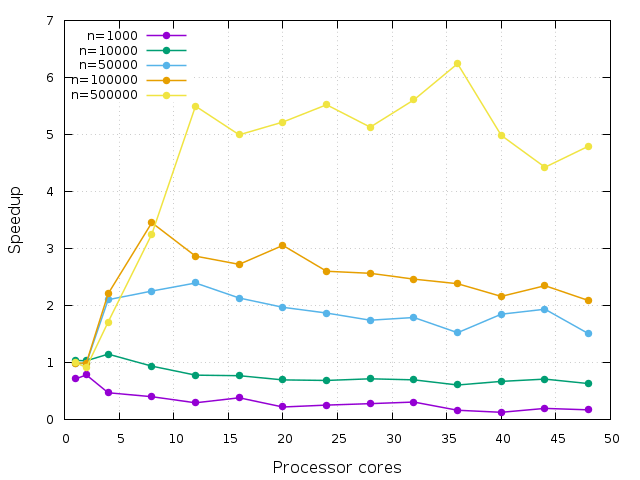
\includegraphics[width=404pt]{resources/plots/Cilk_Disjunct_sizes.png}
	\caption{Cilk (disjuct) - Speedup als Funktion der Prozessorkerne}
	\label{Cilk_Disjunct_sizes}
\end{figure}

\begin{figure}[p]
	\centering
	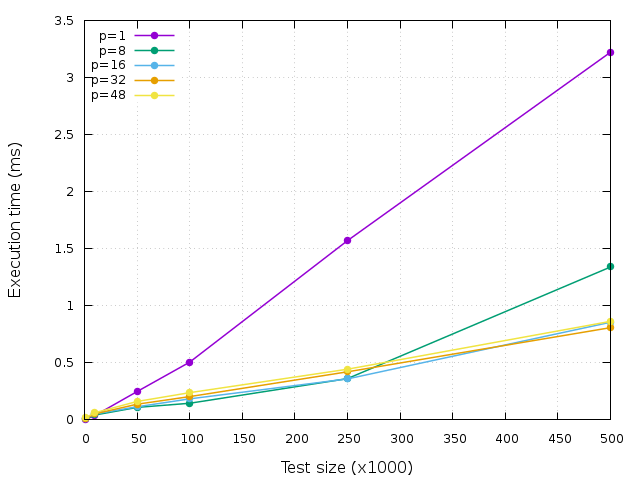
\includegraphics[width=404pt]{resources/plots/Cilk_Disjunct_cores.png}
	\caption{Cilk (disjuct) - Ausführungszeit als Funktion der Testgröße}
	\label{Cilk_Disjunct_cores}
\end{figure}

\begin{figure}[p]
	\centering
	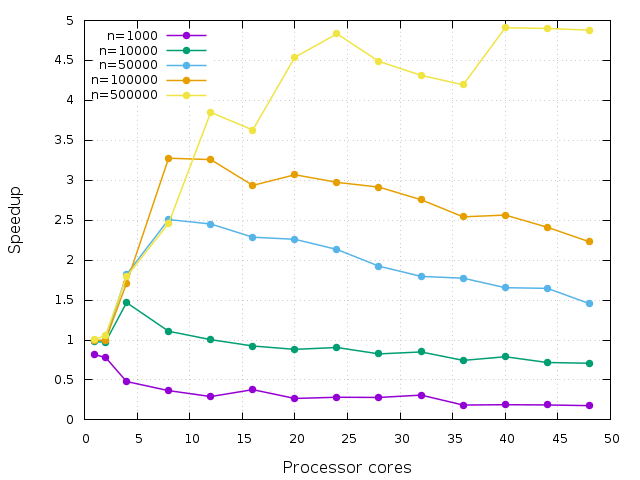
\includegraphics[width=404pt]{resources/plots/Cilk_Interleaved_sizes.png}
	\caption{Cilk (interleaved) - Speedup als Funktion der Prozessorkerne}
	\label{Cilk_Interleaved_sizes}
\end{figure}

\begin{figure}[p]
	\centering
	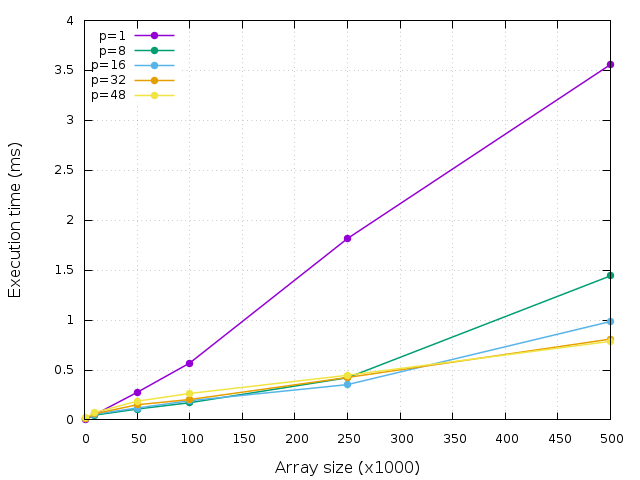
\includegraphics[width=404pt]{resources/plots/Cilk_Interleaved_cores.png}
	\caption{Cilk (interleaved) - Ausführungszeit als Funktion der Testgröße}
	\label{Cilk_Interleaved_cores}
\end{figure}



\subsection{OpenMP}
Im Gegensatz zu Cilk lieferte unsere Implementierung in OpenMP einen erstaunlich großen Speedup.
Sieht man sich die Abbildungen \ref{OpenMP_Disjunct_sizes} und \ref{OpenMP_Interleaved_sizes} an, kann man erkennen, dass der Speedup bei $n = 500000$ einigermaßen linear mit der Anzahl der Threads ansteigt.
In einigen Tests konnte sogar ein superlinearer Speedup erreicht werden.
Natürlich ist so ein Ergebnis in der Theorie nicht möglich.
Eine mögliche Erklärung hierfür ist, dass die Ausführung der sequentiellen Implementierung ungewöhnlich lange gedauert hat, weil die Prozessoren in dieser Zeit gut ausgelastet waren.
Nichtsdestotrotz scheint OpenMP für das gegebene Problem sehr gut geeignet zu sein.
Siehe auch die Abbildungen \ref{OpenMP_Disjunct_sizes}, \ref{OpenMP_Disjunct_cores}, \ref{OpenMP_Interleaved_sizes} und \ref{OpenMP_Interleaved_cores}.

Noch deutlicher als in Cilk sieht man den Unterschied zwischen den beiden Szenarien \emph{Interleaved} und \emph{Disjunct}.
Während der Speedup bei \emph{Disjunct} und $n = 500000$ den Faktor 50 deutlich übersteigt, ist bei \emph{Interleaved} bereits bei etwa 25 Schluss.


\begin{figure}[p]
	\centering
	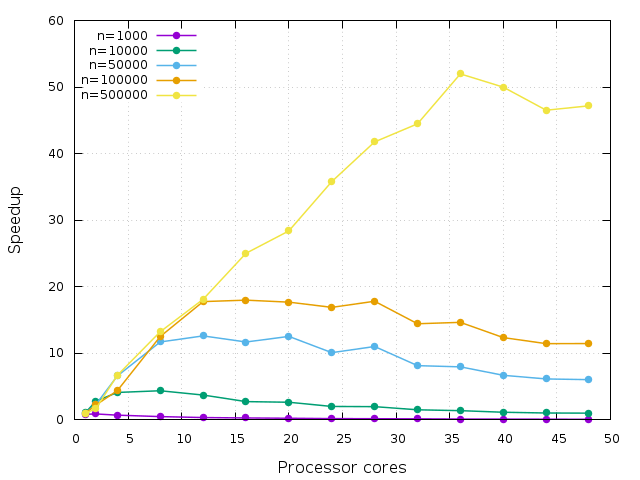
\includegraphics[width=404pt]{resources/plots/OpenMP_Disjunct_sizes.png}
	\caption{OpenMP (disjuct) - Speedup als Funktion der Prozessorkerne}
	\label{OpenMP_Disjunct_sizes}
\end{figure}

\begin{figure}[p]
	\centering
	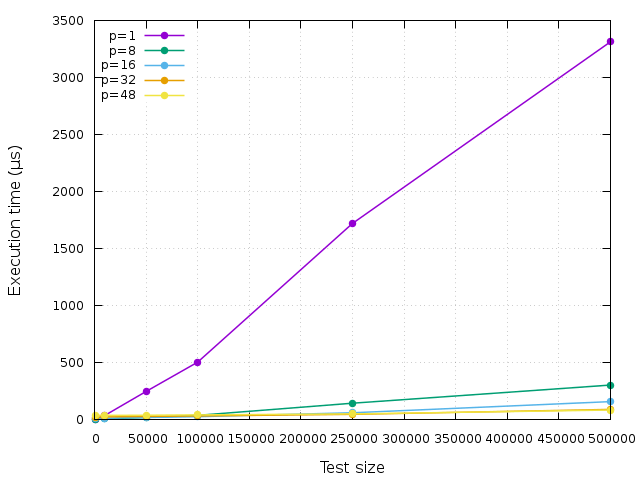
\includegraphics[width=404pt]{resources/plots/OpenMP_Disjunct_cores.png}
	\caption{OpenMP (disjuct) - Ausführungszeit als Funktion der Testgröße}
	\label{OpenMP_Disjunct_cores}
\end{figure}

\begin{figure}[p]
	\centering
	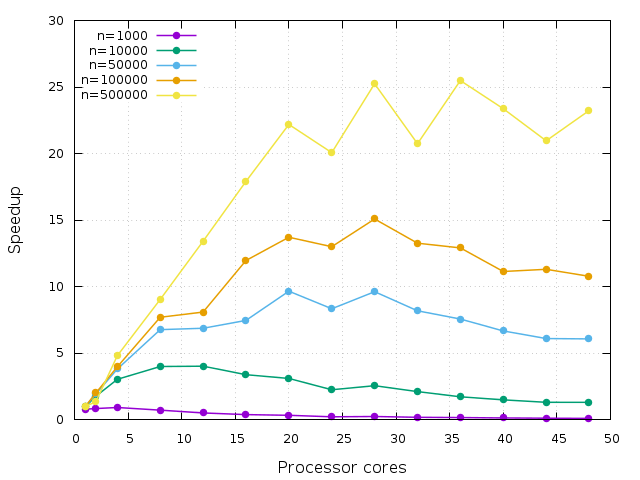
\includegraphics[width=404pt]{resources/plots/OpenMP_Interleaved_sizes.png}
	\caption{OpenMP (interleaved) - Speedup als Funktion der Prozessorkerne}
	\label{OpenMP_Interleaved_sizes}
\end{figure}

\begin{figure}[p]
	\centering
	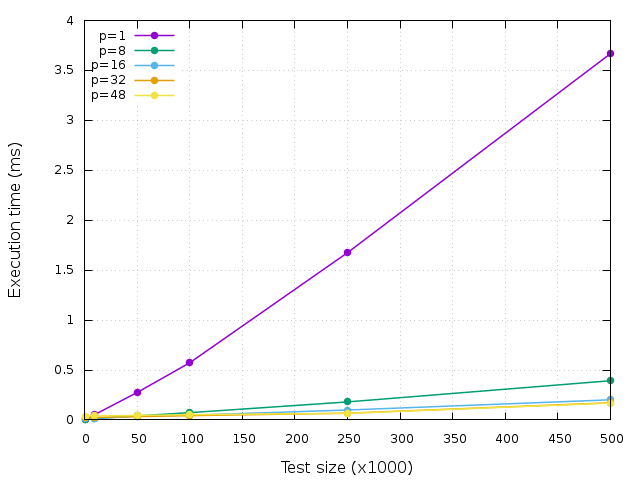
\includegraphics[width=404pt]{resources/plots/OpenMP_Interleaved_cores.png}
	\caption{OpenMP (interleaved) - Ausführungszeit als Funktion der Testgröße}
	\label{OpenMP_Interleaved_cores}
\end{figure}



\subsection{MPI}
Die Benchmarks der MPI-Implementierung haben uns sehr überrascht.
Selbst bei großen Arrays und vielen Prozessoren war nur ein sehr geringer Geschwindigkeitszuwachs zu verzeichnen.
In keinem der getesteten Szenarien kam der Speedup je über den Faktor 3 hinaus.
Spätestens ab einer Prozessorzahl von 100 kam es zudem zu keinem nennenswerten Anstieg der Geschwindigkeit mehr.
Es macht daher praktisch keinen Unterschied, ob 100 oder 500 Kerne zur Lösung des Problems verwendet werden.
Vergleiche hierzu die Abbildungen \ref{MPI_Disjunct_sizes}, \ref{MPI_Disjunct_cores}, \ref{MPI_Interleaved_sizes} und \ref{MPI_Interleaved_cores}.
Wir gehen davon aus, dass der Kommunikationsoverhead bei dem implementierten Algorithmus zu groß ist.


\begin{figure}[p]
	\centering
	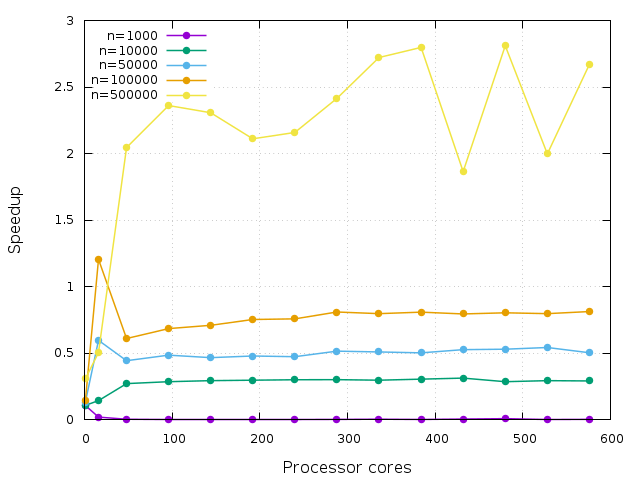
\includegraphics[width=404pt]{resources/plots/MPI_Disjunct_sizes.png}
	\caption{MPI (disjuct) - Speedup als Funktion der Prozessorkerne}
	\label{MPI_Disjunct_sizes}
\end{figure}

\begin{figure}[p]
	\centering
	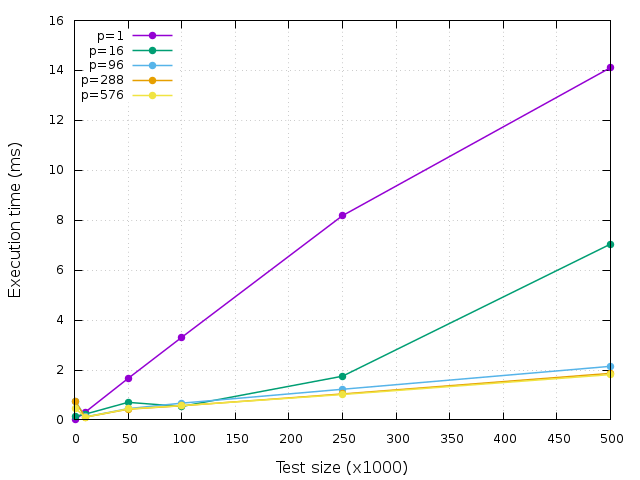
\includegraphics[width=404pt]{resources/plots/MPI_Disjunct_cores.png}
	\caption{MPI (disjuct) - Ausführungszeit als Funktion der Testgröße}
	\label{MPI_Disjunct_cores}
\end{figure}

\begin{figure}[p]
	\centering
	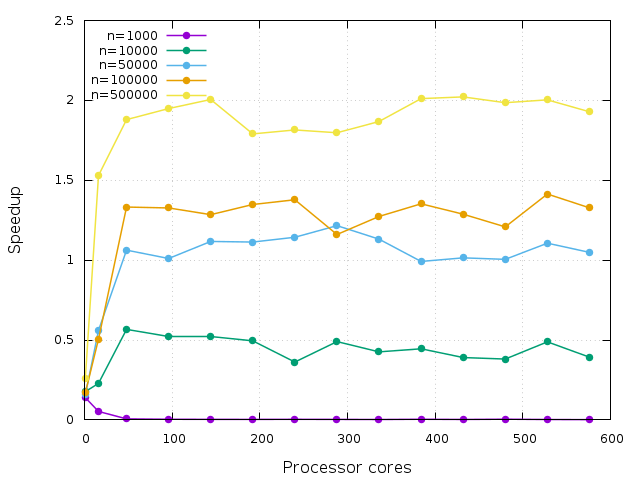
\includegraphics[width=404pt]{resources/plots/MPI_Interleaved_sizes.png}
	\caption{MPI (interleaved) - Speedup als Funktion der Prozessorkerne}
	\label{MPI_Interleaved_sizes}
\end{figure}

\begin{figure}[p]
	\centering
	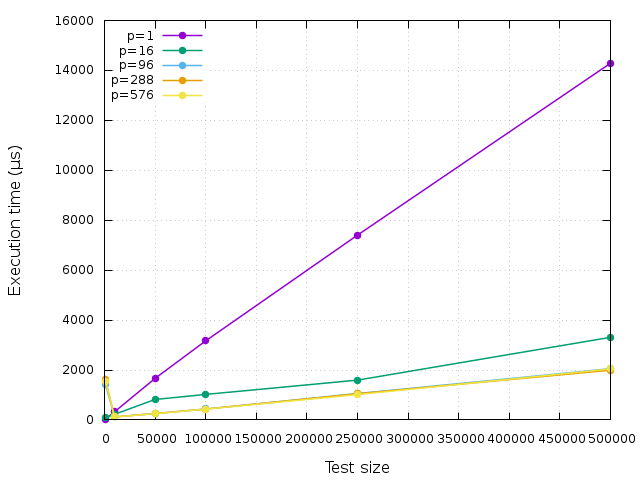
\includegraphics[width=404pt]{resources/plots/MPI_Interleaved_cores.png}
	\caption{MPI (interleaved) - Ausführungszeit als Funktion der Testgröße}
	\label{MPI_Interleaved_cores}
\end{figure}
